\section{Бинарные отношения}
\label{sec:binary_relations}

В данном разделе мы поговорим о некоторого рода обобщении понятия <<функция>>~--- о \defemph{бинарном отношении}.
Напомним, что согласно определению \ref{definition:functions:function} функция $ f $~---
это подмножество некоторого декартового произведения $ X \times Y $,
обладающее свойством \defemph{функциональности}:
\[
    \left[ (x, y) \in f \wedge (x, y') \in f \right] \rightarrow (y = y')
\]
Иначе говоря, любому элементу из $ X $ ставится в соответствее не более одного элемента из $ Y $.
Однако это довольно сильное ограничение.
Например, функциями невозможно описать отношения между некоторыми студентами и их увлечениями:
любой студент вполне может иметь несколько интересных ему занятий,
ровно как и некоторым занятием могут увлекаться несколько человек.

В этой связи в математике отдельно рассматриваются и подмножества $ X \times Y $,
не обязательно обладающие свойством функциональности~--- \defemph{бинарные отношения}.

\begin{definition}
    \label{definition:binary_relations:binary_relation}
    \defemph{Бинарным отношением} между двумя множествами $ A $ и $ B $ называется любое множество $ R \subseteq A \times B $.
    Если $ A = B $, то $ R \subseteq A^2 $ и говорят, что бинарное отношение задано на множестве $ A $.
    Принадлежность $ (a, b) \in R $ кратко записывают как $ a R b $.
\end{definition}

\begin{remark}
    Заметим, что определение \ref{definition:binary_relations:binary_relation} обобщается и на случай произвольного (пусть $ n $) числа множителей в декартовом произведении.
    В таком случае говорят об \defemph{отношении арности $ n $}.
    В нашем курсе мы подробно изучать их не будем.
\end{remark}

Помимо свойства функциональности бинарное отношение может обладать целым набором других интересных свойств.
Перечислим наиболее важные из них:
\begin{definition}
    \label{definition:binary_relations:types_AB}
    Пусть $ R \subseteq A \times B $.
    Отношение $ R $ называется
    \begin{enumerate}
        \item \defemph{функциональным} в случае $ \forall a \in A \;\; \forall b, b' \in B \; \left[ a R b \wedge a R b' \right] \rightarrow (b = b') $.
        \item \defemph{(левым) тотальным} в случае $ \forall a \in A \;\; \exists b \in B: \; a R b $.
        \item \defemph{инъективным} в случае $ \forall a, a' \in A \;\; \forall b \in B \; \left[ a R b \wedge a' R b \right] \rightarrow (a = a') $.
        \item \defemph{сюръективным} в случае $ \forall b \in B \;\; \exists a \in A: \; a R b $.
    \end{enumerate}
\end{definition}
Используя \ref{definition:binary_relations:types_AB}, легко дать определение, например, инъекции,
как функционального тотального инъективного бинарного отношения.

Еще большим числом особых свойств могут обладать бинарные отношения,
заданные на одном множестве.
\begin{definition}
    \label{definition:binary_relations:types_AA}
    Пусть $ R \subseteq A^2 $.
    Отношение $ R $ называется
    \begin{enumerate}
        \item \defemph{рефлексивным} в случае $ \forall a \in A \;\; a R a $.
        \item \defemph{антирефлексивным} в случае $ \forall a \in A \;\; \neg (a R a) $.
        %\item \defemph{корефлексивным} в случае $ \forall a, b \in A \;\; a R b \rightarrow (a = b) $.
        \item \defemph{симметричным} в случае $ \forall a, b \in A \;\; \left( a R b \rightarrow b R a \right) $.
        \item \defemph{антисимметричным} в случае $ \forall a, b \in A \;\; \left[ a R b \wedge b R a \rightarrow (a = b) \right] $.
        \item \defemph{асимметричным} в случае $ \forall a, b \in A \;\; \left[ a R b \rightarrow \neg (b R a) \right] $.
        \item \defemph{транзитивным} в случае $ \forall a, b, c \in A \;\; \left[ a R b \wedge b R c \rightarrow a R c \right] $.
    \end{enumerate}
\end{definition}

\begin{remark}
    Любое рефлексивное бинарное отношение по определению является тотальным и сюръективным.
\end{remark}

Множество уже известных вам математических объектов и операций по сути являются бинарными отношениями.
Например, операции сравнения: $ \{ (a, b) \mid a \, (*) \, b \} \subseteq \R^2 $, где вместо $ (*) $ можно подставить $ <, \leqslant, =, \neq, \geqslant, > $.
Когда рассматривают операции сравнения в терминах бинарных отношений, их обычно заключают в круглые скобки.
Например, $ (<) = \{ (a, b) \mid a < b \} \subseteq \R^2 $.

\begin{Exercise}[counter=SecExercise]
    \noindent
    Какие из указанных в \ref{definition:binary_relations:types_AB} и \ref{definition:binary_relations:types_AA}
    свойств выполнены для следющих бинарных отношений: $ (<), (\leqslant), (=), (\neq), (\geqslant), (>) $?
    Считайте, что $ \R $~--- множество, на котором заданы отношения.
\end{Exercise}

\begin{Answer}
    \noindent
    Нетрудно заметить, что все отношения тотальные и сюръективные.
    Также все отношения, кроме $ (\neq) $, транзитивные.
    Отношение $ (=) $ при этом также функциональное, инъективное, рефлексивное и симметричное.
    Отношение $ (\neq) $ антирефлексивное и симметричное.
    Отношения $ (\leqslant) $ и $ (\geqslant) $ рефлексивные и антисимметричные.
    Наконец, отношения $ (<) $ и $ (>) $ антирефлексивные и асимметричные.
\end{Answer}

Так как бинарные отношения являются множествами, к ним применимы теоретикомножественные операции:
отношения можно объединять, пересекать, вычитать, брать дополнение к ним и так далее.
Однако этим операции над бинарными отношениями не ограничиваются.

\begin{definition}
    \defemph{Обратным отношением} к бинарному отношению $ R \subseteq A \times B $ называется отношение
    $ R^{-1} = \{(b, a) \mid a R b \} \subseteq B \times A $.
\end{definition}

\begin{Exercise}[counter=SecExercise, label={exercise:relations:is_function}]
    \noindent
    Нарисуйте двудольный граф, соответсвующий бинарному отношению
    $ R \subseteq \{a, b, c, d, e\} \times \{1, 2, 3, 4, 5, 6\} $:
    \[
        R = \{ (a, 1), (a, 2), (b, 4), (c, 3), (d, 5) \}
    \]
    \begin{enumerate}[label=\textbf{\alph*)}]
        \item Является ли $ R $ функцией?
        \inlineitem Является ли $ R^{-1} $ функцией?
    \end{enumerate}
\end{Exercise}

\begin{Answer}
    \noindent
    Граф приведён на рисунке \ref{fig:relations:from_is_function}.
    \begin{enumerate}[label=\textbf{\alph*)}]
        \item
            Нет, не является, так как $ (a, 1) \in R $ и $ (a, 2) \in R $.
        \item
            Да, является, так как $ \forall b \in \{1, \ldots, 6 \} $
            множество $ \{ a \mid b R^{-1} a \} $ содержит не более одного элемента.
    \end{enumerate}
\end{Answer}

\begin{figure}[ht!]
    \center
    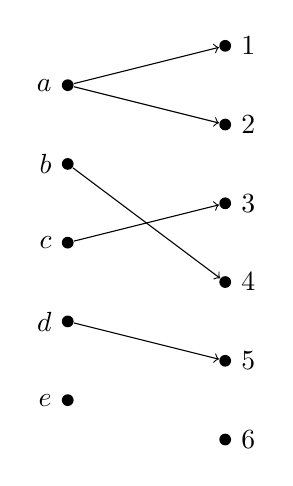
\begin{tikzpicture}
        \node[circle,fill,inner sep=1.5pt,label=left:$ a $] (a)  at (0,-0.5) {};
        \node[circle,fill,inner sep=1.5pt,label=left:$ b $] (b)  at (0,-1.5) {};
        \node[circle,fill,inner sep=1.5pt,label=left:$ c $] (c)  at (0,-2.5) {};
        \node[circle,fill,inner sep=1.5pt,label=left:$ d $] (d)  at (0,-3.5) {};
        \node[circle,fill,inner sep=1.5pt,label=left:$ e $] (e)  at (0,-4.5) {};

        \node[circle,fill,inner sep=1.5pt,label=right:$ 1 $] (u1)  at (2,0) {};
        \node[circle,fill,inner sep=1.5pt,label=right:$ 2 $] (u2)  at (2,-1) {};
        \node[circle,fill,inner sep=1.5pt,label=right:$ 3 $] (u3)  at (2,-2) {};
        \node[circle,fill,inner sep=1.5pt,label=right:$ 4 $] (u4)  at (2,-3) {};
        \node[circle,fill,inner sep=1.5pt,label=right:$ 5 $] (u5)  at (2,-4) {};
        \node[circle,fill,inner sep=1.5pt,label=right:$ 6 $] (u6)  at (2,-5) {};

        \path [->] (a) edge node {}  (u1);
        \path [->] (a) edge node {}  (u2);
        \path [->] (b) edge node {}  (u4);
        \path [->] (c) edge node {}  (u3);
        \path [->] (d) edge node {}  (u5);
    \end{tikzpicture}
    \caption{граф отношения $ R $ из задачи \ref{exercise:relations:is_function}}
    \label{fig:relations:from_is_function}
\end{figure}


\begin{definition}
    \defemph{Композицией} двух бинарных отношений $ R \subseteq A \times B $ и $ Q \subseteq B \times C $
    называется бинарное отношение $ (Q \circ P) = \{ (a, c) \mid \exists b \in B: \; a R b \wedge b Q c \} $.
    %\newline
    \\[0.25\baselineskip]
    Акцентируем особое внимание на порядок записи отношений в композиции.
    Он повторяет порядок записи функций в композиции.
\end{definition}

\begin{Exercise}[counter=SecExercise]
    \noindent
    Найдите результат операций над отношениями, определенными на множестве действительных чисел.
    \begin{enumerate}[label=\textbf{\alph*)}]
        \item $ (>)^c $;
        \inlineitem $ (>)^{-1} $;
        \inlineitem $ (\geqslant) \symdiff (\leqslant) $;
        \inlineitem $ (>) \cap (<) $;
        \inlineitem $ (=) \circ (>) $;
        \inlineitem $ (<) \circ (<) $;
        \item $ (<) \circ (>) $.
    \end{enumerate}
\end{Exercise}

\begin{Answer}
    \noindent
    \begin{enumerate}[label=\textbf{\alph*)}]
        \item $ (\leqslant) $;
        \inlineitem $ (<) $;
        \inlineitem $ (\neq) $;
        \inlineitem $ \varnothing $;
        \inlineitem $ (>) $;
        \inlineitem $ (<) $;
        \inlineitem $ \R^2 $;
    \end{enumerate}
\end{Answer}


\subsection{Отношения эквивалентности}
\label{subsec:binary_relations:equivalency}

Отношения подобия треугольников или параллельности прямых также являются бинарными отношениями.
Можно заметить, что оба этих отношения (если считать прямую параллельной самой себе)
вместе с отношением $ (=) $ и многими другими являются рефлексивными, симметричными и транзитивными.
Такие отношения выделяют в отдельную группу.

\begin{definition}
    Рефлексивное, симметричное и транзитивное бинарное отношение называют \defemph{отношением эквивалентности}.
\end{definition}

\begin{theorem}
    \label{theorem:binary_relations:eq_classes_partition}
    Пусть на конечном множестве $ A $ задано отношение эквивалентности $ R $.
    Тогда $ A = B_1 \sqcup B_2 \sqcup \ldots \sqcup B_k $,
    причём $ \forall i \; B_i \neq \varnothing $ и $ \forall a \in B_i \; \forall b \in B_j \; \left[ a R b \leftrightarrow (i = j) \right] $.
    То есть, два элемента образуют пару, лежащую в отношении, тогда и только тогда, когда они взяты из одного блока разбиения.
\end{theorem}

\begin{remark}
    Теорема \ref{theorem:binary_relations:eq_classes_partition} справедлива и для бесконечных $ A $.
    Тогда число блоков не обязательно конечно или даже счётно.
\end{remark}

\begin{definition}
    Блоки $ B_i $ из \ref{theorem:binary_relations:eq_classes_partition} называются \defemph{классами эквивалентности},
    а про $ A $ говорят, что оно разбито на классы эквивалентности.
\end{definition}

Из теоремы \ref{theorem:binary_relations:eq_classes_partition} следует,
что для любого элемента $ A $ однозначно определён класс эквивалентности, в котором данный элемент лежит.
В связи с этим получаем эквивалентное определение класса эквивалентности:

\begin{definition}
    Пусть $ R \subseteq A^2 $~--- отношение эквивалентности, $ a \in A $.
    Тогда \defemph{классом эквивалентности} отношения $ R $, построенным по представителю $ a $ называется множество
    $ [a]_R = \{ b \in A \mid a R b \} $.
\end{definition}

\begin{corollary}
    Любые два класса эквивалентности либо совпадают, либо не пересекаются:
    $ \forall a, b \in A \;\; ([a]_R = [b]_R) \oplus ([a]_R \cap [b]_R = \varnothing) $.
\end{corollary}

\begin{Exercise}[counter=SecExercise]
    \noindent
    Рассмотрим множество $ S $ фундаментальных последовательностей, состоящих из рациональных чисел.
    Введём следующее бинарное отношение $ (\sim) \subseteq S^2 $:
    \[
        \{x_i\}_{i = 1}^{\infty} \sim \{y_j\}_{j = 1}^{\infty}
        \quad \Longleftrightarrow \quad
        \forall \varepsilon > 0 \;\; \exists N \in \N: \forall n,m > N \;\; |x_n - y_m| < \varepsilon
    \]
    Является ли $ (\sim) $ отношением эквивалентности?
\end{Exercise}

\begin{Answer}
    \noindent
    Симметричность очевидным образом следует из симметричности формулы в условии.
    Рефлексивность эквивалентна фундаментальности любой последовательности из $ S $ (совпадение с определением буквальное),
    что дано по условию.
    Осталось проверить транзитивность.
    Для этого достаточно взять $ \varepsilon' = \varepsilon / 2 $ и воспользоваться неравенством треугольника:
    \begin{multline*}
        \left .
        \begin{aligned}
            \forall n,k > N_1(\varepsilon') \;\; |x_n - y_k| < \varepsilon' \\
            \forall k,m > N_2(\varepsilon') \;\; |y_k - z_m| < \varepsilon'
        \end{aligned}
        \right \}
        \quad \Longrightarrow \quad
        \forall n, m, k > \max\{N_1, N_2\} \;\; |x_n - z_m| = \\
        = |x_n - y_k + y_k - z_m| < |x_n - y_k| + |y_k - z_m| < 2 \varepsilon' = \varepsilon
    \end{multline*}
    Отсюда имеем транзитивность.

    Интересно, что для классов эквивалентности рассматриваемого отношения можно ввести стандартные математические операции
    (например, $ [\{x_i\}_{i=1}^{\infty}]_{(\sim)} + [\{y_i\}_{i=1}^{\infty}]_{(\sim)} = [\{x_i + y_i\}_{i=1}^{\infty}]_{(\sim)} $;
    проверьте непротиворечивость такого определения).
    Более того, после этого классы приобретаеют свойства \emph{действительных чисел}.
    Можно в некотором смысле саказать, что это и есть все действительные числа (см. \emph{изоморфизм}).
\end{Answer}


\subsection{Отношения частичного порядка}
\label{subsec:binary_relations:order}

В прошлом разделе мы упомянули один из важнейших классов бинарных отношений, представители которого по свойствам близки к отношению равенства.
Логично предположить, что и у других изученных бинарных отношениях на числах есть аналогичные <<братья>>.
Действительно, можно, например, заметить, что у отношений $ (\leqslant) $ и $ (\subseteq) $\footnote{не будем пока формально определять, на чём они заданы}
много общих свойств: оба отношения \emph{рефлексивные}, \emph{антисимметричные} и \emph{транзитивные}.
Также, например, $ (<) $ и $ (\subsetneq) $ \emph{антирефлексивные}, \emph{антисимметричные} и \emph{транзитивные}.
Такие отношения также выделяют в отдельную группу.

\begin{definition}
    Транзитивное, антисимметричное и \underline{либо} рефлексивное, \underline{либо} антирефлексивное бинарное отношение называют \defemph{отношением (частичного) порядка}.
    %\newline
    В случае рефлексивности говорят, что отношение порядка \defemph{нестрогое}, иначе~--- \defemph{строгое}.
\end{definition}

\begin{remark}
    \label{remark:binary_relations:order_bijection}
    Из любого отношения нестрогого порядка можно получить строгое, вычтя из него отношение $ (=) $ как множество.
    Аналогично можно совершить и обратное преобразование.
    Таким образом, между множеством строгих и нестрогих порядков определена биекция.
\end{remark}

\begin{definition}
    Пусть $ R $~--- отношение частичного порядка.
    Будем обозначать $ (<_R) $ и $ (\leqslant_R) $ строгую и нестрогую версию $ R $ соответственно,
    полученные согласно биекции из \ref{remark:binary_relations:order_bijection}.
    \textit{Во избежание путанницы заметим, что хотя бы с одной из этих версий $ R $ совпадает по определению.}
\end{definition}

\begin{definition}
    Отношения порядка, в которых любые два элемента сравнимы (то есть $ \forall a \forall b \in A \; \left[a R b \vee b R a \right]$),
    называются \defemph{линейными}.
    Заметим, что линейными могут быть только отношения нестрогого порядка.
\end{definition}

В некоторых задачах исследование отношения порядка может быть неудобным из-за большого числа <<неинфомативных>> пар.
Например, отношение $ (<) $ на $ \Z $ однозначно задаётся парами вида $ (n, n+1) $ и знанием о его транзитивности и линейности;
необязательно рассматривать все пары, для того чтобы полностью восстановить всё отношение.
В связи с этим вводится следующее понятие:

\begin{definition}
    Пусть $ R \subseteq A^2 $~--- отношение частичного порядка.
    Отношением \defemph{непосредственного следования}, построенным по $ R $, является бинарное отношение
    \[
        (\prec_R) = \left\{ (x, y) \mid (x <_R y) \wedge \neg \left( \exists z \in A: (x <_R z) \wedge (z <_R y) \right) \right\}
    \]
\end{definition}

Название отношения полностью соответствует его определению.
Рассмотрим несколько примеров:

\begin{example}
    \begin{enumerate}
        \item[]
        \item
            Рассмотрим $ (<) \subseteq \Z^2 $.
            Тогда $ \prec_{(<)} = \left\{ (n, n+1) \mid n \in \Z \right\} $.
        \item
            Рассмотрим $ (<) \subseteq \R^2 $.
            Из плотности действительных чисел самих в себе следует, что $ \prec_{(<)} = \varnothing $.
            Это действительно согласуется с интуицией: ни для какого действительного числа нельзя назвать другое,
            следующее непосредственно за ним.
        \item
            Рассмотрим $ (\subsetneq) \in \mathcal{S}^2 $, где $ \mathcal{S} $~--- некоторое семейство множеств.
            Тогда
            \[
                \prec_{(\subsetneq)} = \left\{ (x, y) \mid (x \subseteq y) \wedge (|y \setminus x| = 1) \right\}
            \]
            Видно, что полученное отношение не обязательно функционально или инъективно:
            у множества может быть несколько непосредственно следующих после него множеств;
            точно так же и наоборот.
    \end{enumerate}
\end{example}

\begin{definition}
    Пусть $ R \subseteq A^2 $~--- отношение частичного порядка.
    Ориентированный граф $ G(A, \prec_R) $ называется \defemph{диаграммой Хассе} отношения $ R $.
\end{definition}

\begin{definition}
    Диаграмма Хассе, построенная для частичного порядка $ (\subseteq) \subseteq 2^A \times 2^A $, где $ |A| = n < \infty $,
    называется \defemph{ориентированным булевым кубом}.
    Его неориентированная версия называется просто \defemph{булевым кубом} и обозначается $ B_n $.
    %\newline
    %\textit{Отметим, что это эквивалентное определение, а каноническое будет дано ниже.}
\end{definition}

\begin{remark}
    Вершины булева куба обычно обозначают двоичными словами длины $ n $,
    являющимися векторами значений индикаторных функций соответствующих подмножеств
    ($ i $-ый бит отвечает за наличие $ i $-ого элемента $ A $ в соответствующем подмножестве).
\end{remark}

\begin{figure}[ht!]
    \center
    \begin{tikzpicture}[
    back line/.style={densely dotted},
    cross line/.style={preaction={draw=white, -,
    line width=6pt}}]
        \matrix (m) [matrix of math nodes,
        row sep=3em, column sep=3em,
        text height=1.5ex,
        text depth=0.25ex]{
        & 110 & & 111 \\
        100 & & 101 \\
        & 010 & & 011 \\
        000 & & 001 \\
        };
        \path[->] (m-4-1) edge (m-2-1);
        \path[->] (m-2-1) edge (m-1-2);
        \path[->] (m-1-2) edge (m-1-4);

        \path[->] (m-2-1) edge (m-2-3);
        \path[->] (m-2-3) edge (m-1-4);

        \path[->] (m-4-1) edge (m-4-3);
        \path[->] (m-4-3) edge (m-3-4);
        \path[->] (m-3-4) edge (m-1-4);

        \path[->] (m-4-1) edge [back line] (m-3-2);
        \path[->] (m-3-2) edge [back line] (m-3-4);

        \path[->] (m-3-2) edge [back line] (m-1-2);
        \path[->] (m-4-3) edge (m-2-3);
        %(m-2-3) edge [cross line] (m-4-3);
    \end{tikzpicture}
    \label{fig:binary_relations:boolean_cube}
    \caption{пример ориентированного булева куба для $ n = 3 $.}
\end{figure}

На практике часто встречаются задачи, в которых надо ввести частичный порядок на некотором декартовом произведении.
При этом на множителях обычно некоторый порядок уже введён.
В этих случаях удобна следующая конструкция:

\begin{definition}
    Пусть $ P \subseteq A^2 $, $ Q \subseteq B^2 $~--- отношения порядка.
    Их \defemph{произведением} называется бинарное отношение $ P \subseteq (A \times B)^2 $:
    \[
        (x, y) \, P \, (x', y') \; \Longleftrightarrow \;
        \begin{cases}
            x R x' \\
            y Q y'
        \end{cases}
    \]
    Вводится следующее обозначение: $ P = A \times B $, хотя, формально, с точки зрения множеств оно означает другое.
\end{definition}

Заметим, что произведение отношения порядков не всегда является отношеним порядка.
Для этого требуется, чтобы множители были либо одновременно нестрогими порядками, либо строгими.

\begin{remark}
    \label{remark:binary_relations:boolean_cube_isomorphism}
    Ориентированный булев куб также является диаграммой Хассе для отношения порядка
    $ (\leqslant \times \leqslant \times \ldots \times \leqslant) \subseteq \{ 0, 1 \}^n \times \{ 0, 1 \}^n $~---
    \defemph{отношения покоординатного порядка}, введённого на двоичных словах длины $ n $.
    Обратим внимание, что \textbf{\uline{это каноническое определение булева куба в нашем курсе}}.
\end{remark}

Данное замечание хорошо иллюстрируется следующей задачей:
\begin{Exercise}[counter=SecExercise]
    \noindent
    Граф $ G_n = (V, E) $ имеет множество вершин $ V = 2^{\{1, 2, \ldots, n\}} $
    (вершина $ v \in V $~--- подмножество множества $ \{1, 2, 3, \ldots, n \} $);
    вершины $ v $ и $ u $ соединены ребром тогда и только тогда, когда $ | u \symdiff v | = 1 $.
    \begin{enumerate}[label=\alph*)]
        \item
            Докажите, что граф $ G_n $ изоморфен булеву кубу $ B_n $.
        \item
            Сколько существует различных наборов (попарно различных) подмножеств $ A_1, A_2, A_3 \subseteq \{1, 2, \ldots, n\} $,
            для которых выполняется условие $ |A_1 \symdiff A_2| = |A_2 \symdiff A_3| = 1 $?
    \end{enumerate}
\end{Exercise}

\begin{Answer}
    \noindent
    \begin{enumerate}[label=\alph*)]
        \item
            Изоморфизм, по сути, уже построен в замечании \ref{remark:binary_relations:boolean_cube_isomorphism}:
            действиетльно, любому подмножеству $ A \subseteq V $ взаимнооднозначно сопоставляется двоичное слово длины $ |V| $ (вектор значений индикаторной функции),
            причём $ A_1 \subseteq A_2 $ тогда и только тогда, когда вектор, соответствующий $ A_1 $,
            сравним по отношению покоординатного порядка с вектором, соответвтующим $ A_2 $,
            и покоординатно не больше его.
            Убирая ориентацию рёбер, мы не нарушаем изоморфизм.
            Что и требовалось доказать.
        \item
            В силу предыдущего пункта задача эквивалентна поиску путей длины два в булевом кубе.
            Так как всего вершин $ 2^n $, а степень каждой вершины в $ B_n $ равна $ n $, таких путей~--- $ \frac{1}{2} \cdot 2^n \cdot A_n^2 $
            (делим на два так как посчитали каждый путь дважды).
            То есть, ответ~--- $ N = n (n-1) 2^{n-1} $.
    \end{enumerate}
\end{Answer}

Введём, наконец, некоторый дополнительный глоссарий, связанный с отношениями порядка.

\begin{definition}
    \label{definition:binary_relations:max}
    Рассмотрим отношение частичного порядка $ R \subseteq A^2 $.
    Элемент $ x \in A $ является
    \begin{enumerate}
        \item
            \defemph{максимальным} в случае $ \neg \left[ \exists a \in A: (x <_R a) \right] $.
        \item
            \defemph{наибольшим} в случае $ \forall a \in A \; (a \leqslant_R x) $.
    \end{enumerate}
    Аналогично определяются \defemph{минимальный} и \defemph{наименьший} элементы.
\end{definition}

\begin{remark}
    \label{remark:binary_relations:minimal}
    Наибольший/наименьший элемент обязательно является максимальным/минимальным.
\end{remark}

\begin{proof}
    Действительно, предположим противное: есть наибольший, но не максимальный по отношению порядка $ R \subseteq A^2 $ элемент $ x $.
    Тогда, отрицая максимальность, имеем $ \exists a \in A: (x <_R a) $.
    Но в силу антисимметричности $ R $ тогда не может быть, чтобы $ a \leqslant_R x $.
    Противоречие с максимальностью.
    Аналогично для наименьшего элемента.
\end{proof}

\begin{Exercise}[counter=SecExercise]
    \noindent
    Постройте отношение частичного порядка, в котором деревья (и только они) на некотором наборе вершин $ V $ будут минимальными элементами.
    Существуют ли для этого отношения наименьшие элементы?
\end{Exercise}

\begin{Answer}
    \noindent
    Рассмотрим $ A = \left\{ G(V, E) \mid \left( E \subseteq \binom{V}{2} \right) \wedge (G \; \textnormal{связный} ) \right\} $.
    Отношение введём следующим образом: $ R = \left\{ (G, G') \mid E(G) \subseteq E(G') \right\} $.
    Нетрудно заметить, что это отношение нестрогого частичного порядка, так как таковым является $ (\subseteq) $.

    В терминах введённого отношения определение минимального элемента эквивалентно определению дерева:
    связный граф, удаление любого ребра из которого нарушает связность, что эквивалентно связному графу,
    для которого не существует связного подграфа на тех же вершинах.

    Наименьшего элемента в общем случае нет: если $ |V| > 2 $, то может быть построено несколько деревьев.
    Так как это все минимальные элементы, среди них согласно \ref{remark:binary_relations:minimal} и надо искать наименьший элемент.
    Но понятно, что любые два разных дерева не сравнимы.
    Значит, наименьшего элемента нет.
\end{Answer}

В предыдущей задаче мы ввели отношение порядка, которое, вообще говоря, может быть задано на всех графах с вершинами $ V $, а не только на связных.
Здесь логично ввести следующее определение:

\begin{definition}
    Пусть бинарное отношение $ R $ задано на множестве $ A $.
    Пусть $ B \subseteq A $.
    Тогда $ R \cap B^2 $ является бинарным отношением, заданным на множестве $ B $,
    и называется \defemph{сужением} $ R $ на $ B $.
\end{definition}

В связи с этим определением аналогично \ref{definition:binary_relations:max} вводятся понятия максимального,
минимального, наибольшего и наименьшего элемента в подмножестве.
